%\documentclass[Journal,InsideFigs, DoubleSpace]{ascelike} %figs inside
 \documentclass[Journal, BackFigs,NoLists, DoubleSpace]{ascelike}%figs in the back
 %NewProceedings, Journal

%include package for inserting picture
\usepackage{graphicx}%insert image
\DeclareGraphicsExtensions{.pdf,.png,.jpg}
\graphicspath{{figures/}}%folder contains images

\usepackage{caption}%packages for inserting multiple pictures
\usepackage{subcaption}%packages for inserting multiple pictures

\usepackage{array}%for table with fixed width
\newcolumntype{L}[1]{>{\raggedright\let\newline\\\arraybackslash\hspace{0pt}}m{#1}}
\newcolumntype{C}[1]{>{\centering\let\newline\\\arraybackslash\hspace{0pt}}m{#1}}
\newcolumntype{R}[1]{>{\raggedleft\let\newline\\\arraybackslash\hspace{0pt}}m{#1}}

\usepackage{amsmath} %math package

\usepackage{algorithm} %algorithm package
\usepackage[noend]{algpseudocode} % pseudo code package

\usepackage[utf8]{inputenc}%french accents
\usepackage[T1]{fontenc} %for accented characters

\usepackage{booktabs}%allowing drawing hline in table crossing only some columns

\usepackage{enumitem}


\begin{document}

\title{NLP-based approach to classify heterogeneous terms \\for unambiguous exchange of roadway data}

% automated generation of highway lexicon classifying lexical relationships between heterogeneous highway technical terms lexicon generation , inconsistency  \\in highway projects}

%
\author{
Tuyen Le
\thanks{
Ph.D. Candidate, Department of Civil, Construction and Environmental Engineering, Iowa State University. Ames, IA 50011, United States. E-mail: ttle@iastate.edu.},
\and
H. David Jeong
\thanks{Associate Professor, Department of Civil, Construction and Environmental Engineering, Iowa State University. Ames, IA 50011, United States. E-mail: djeong@iastate.edu.}
 }

\maketitle
%
%\begin{center}
%(To be submitted to the Journal of Computing in Civil Engineering) 
%\end{center}

\begin{abstract} %150-175 words (as required by ASCE)
%background:
The inconsistency of data terminology due to the fragmented nature of the highway industry has imposed big challenges on integrating digital data from distinct sources. The issue of semantic heterogeneity may lead to the lack of common understanding of the same data between the sender and receiver. Explicit semantic relations among terms in digital dictionaries, such as ontologies can enable the meaning of a roadway concept name to be transparent and unambiguously understood by computer systems. However, due to the lack of an effective automated method, current practices of identifying these relations hardly rely on a manual process of knowledge acquisition from domain experts or text documents which is laborious and time-consuming.
%research objective
This paper presents a novel methodology that leverages recent advances in Natural Language Processing (NLP) techniques to extract English-American roadway terms used in different government agencies and their semantic relations from roadway design manuals and specifications.
%research methods
The proposed method includes the following three stages: (1) implement NLP techniques to detect commonly used technical terms from the highway corpus; (2) utilize machine learning to learn the semantic similarity among roadway terms using their context data in the corpus; and (3) design a classification algorithm to identify semantic relation types among technical terms.
%research value
The key merit in this technique is the automated identification of semantic relations among heterogeneous roadway terms from design guidebooks without reliance on other existing hand-coded semantic resources.
%result
The proposed methodology was evaluated by conducting an experiment comparing the automatically-identified synonyms by the proposed system with a human-constructed golden standard dataset obtained from Wikipedia. The result shows that the proposed model achieves a precision of over 80 percent.
  
\end{abstract}

\KeyWords{Roadway Data, Semantic Relation, Data Sharing, Semantic Interoperability, Natural Language Processing, Vector Space Model}
%
%\newpage


%***********good terms and phrases:*********************************************
%other resources to find context words:
%---R1: http://skell.sketchengine.co.uk/run.cgi/skell
%---R2: http://corpus.byu.edu/coca/
%---R2: http://www.just-the-word.com/

%--------------------************************---------------------------------------

%---adj01: many, plenty, a plethora, a few, very few, various, variety of , large body of research on, very little of st, a lack of, shortcoming, 
%---adj02: main, key, major, principle, primary, secondary, minor, critical, strategic, insightful, enabling technologies,  popular, mature, play a central role, notable, cutting-edge, 
%---adj03: nonhierarchical, superior, well-defined; foreseeable; disparate, isolated,, proprietary, integrated, shared, sharable, inefficient,  consistent,  intuitive solutions,  transformative impact,
%---adj04: inexpensive, easy-to-use, time and cost-efficient,  laborious and resource-intensive, labour extensive, rigorous, ad-hoc, time-consuming, laborious, prone error, human effort, 
%---adj05: empirical work, automated, 
%---adj06: rigid, flexible
%---adj07: proper, precise, right, successful
%---adj08: specialized, special, typical
%---adj09: inconsistent (inconsistency)
%---adj10: effective (effectiveness)
%---adj11: advanced (advancement, advantages)
%---adj12: concise (concisely)
%---adj13: broad, narrow, specific, typical, particular
%---adj14: 


%--------------------************************---------------------------------------

%---noun1: challenges, barrier, hinders, obstacles, impediment; that approximate concepts; extraction=deduction=acquisition; broad spectrum; overtake these technical and economic challenges; bottleneck; data creation and utilization; in the midst of planning; interpretation; multitude of data,  data repository, a structured system of terms, data representation, initiatives, bottleneck, insight and value from massive amounts of data, technology and skillset, data scale, magnitude,  a plethora of, data sharing paradigm, discrepancy, the origin of, vicinity=neighborhood, 
%---noun2: solution, method, 
%---noun3: human effort
%---noun4: outcome, deliverable, result, 
%---noun5: discipline, agency, organization, stakeholder, partner
%---noun6: staff, personnel, industry expert, practitioner, academic community, researchers, professionals, 
%---noun7: stage, phase, 
%---noun8: process, timeframe, procedure, 
%---noun9: technology, tool, technique, product, engine, 
%---noun10: goal, purpose, target, aim, finding, result, 
%---noun11: member, constituent, 
%---non12: indicator, determinant, reason, 

%--------------------************************---------------------------------------

%---verb1: tackle, resolve, handle, address, foster, amplified; simplified; detect; aggregate; encompass, manifest, envision,  is divided into two, share (shared),  
%---verb2: affect, impact, influence, trigger, create, transform (transformative), enable (enabler, enabling), allow, support (supporting), ensure, generate (generation), result in, improve, facilitate, underpin (underpinning), adjust, tailor, accommodate, modify, change, redefine, lead to, cause, implicate (implication), degrade, reduce, decrease, increase
%---verb3: suggest (suggestion), argue, show, explain (explanation), propose, develop (development), examine (examination), investigate (investigation), infer (inference), interpret (interpretation), deliver (deliverable), indicate (indicator, indication), present, find (finding), explore (exploration), recognize (recognition), recommend (recommendation)
%---verb4: use, employ, deploy, implement (implementation), utilize, apply (application), leverage, 
%---verb5: guide, drive, trend, 
%---verb6: involve (involvement), constitute (functions constituting the process), include, encompass, participate (participation), contribute, exclude, limit, cut, consist, comprised, 
%---verb7: require
%---verb8: refer, relate, mention, enumerate, define, 
%---verb9: derive, extract (extraction)
%---verb10: expect, help, 
%---verb11: divide, classify, 
%---verb12: aim (aim), target, is to, seek, 
%---verb13: measure, estimated, compute, quantify, 
%---verb14: vary, differ, 

%--------------------************************---------------------------------------

%---adv: namely, undoubtedly, oftentimes, cohesively, extensively, 

%--------------------************************---------------------------------------

%---linking1: thereby, only those concepts that, whereby, lastly, subsequently, accordingly
%---linking2: technically, basically, theoretically, 
%---linking3: as reported by the FAA, Regarding X, As regards X, In terms of X, In the case of X, With regard to X, With respect to X, In addition, it is important to, From the previous discussion, A comparison of the two results reveals that, This section has reviewed, 
%---linking4: therefore, thus, as a result, 
%---linking5: An notable/important example of this, Examples of this include, For example, X is a good illustration for, This can be illustrated by, By way of illustration, Le (2016), 

%--------------------************************---------------------------------------

%---good phrases: tailored with respect to their context---includes three phases, namely AA, BB and CC--- at such places as parks, fairgounds or town spuares---case-specific developments; area of interests--- incrementally built--- inexpensive and easy-to-use testing device---; time and cost-efficient way--- research community---one of..since then is the--- RDF structure..to make assertion about a resource--- syntax-centered NLP---  such as A, B, etc.--- ..is in it's reliance upon the presence..which is..--- with the objectives of disambiguation--- has triggered a mounting awareness--- to be the main impediment to the progress--- ..start point for deducing other truth-- there is a large body of research on--- see e.g. [2], [14] and [32]--- the former, the latter--- rigorously formalized---- backbone structure of st.---was opted to--- Sections 4.5 and 4.6---- (e.g., Neo4J, OrientDB, Titan)--- forthcoming year--- well-designed process--- is subject to do st.--- in turn means that--- discussion by academics and professionals--- some insights on planning, management, and control--- strategic framework--- in-depth project performance--- in lieu of-- the following expression denotes---is presented/defined as follows--- this/below example shows--- the snippet below presents--- the following is the short description of the rule--- an OWL ontology describing an ifcwindow class--- these concepts and relationships can be encoded in the following RDF/XML fragment--- is written in Turtle syntax/format---formality of representation--- axiomatic richness--- the tool is meant to assess --- it should be..;however, at present, it is not the case --- in conjunction with---it can have good impact when ued in ---

%--------------------************************---------------------------------------

%---sentence structure:  this is evidenced by the accelerating emergence of ...; there is recogintion that 

%********************************************************

\section{Introduction}%900 words
%what is this?-Topic introduction, territory: centrality--> general background information 
%the background of data interoperability
The implementation of advanced, and computerized technologies such as 3D modeling and Geographic Information System (GIS) throughout the life cycle of a highway project has allowed a large portion of project data to be available in a digital format. The efficiency improvement in sharing these data between project participants and stages, will in turn, translate into increased productivity, efficiency in project delivery and accountability. The interoperability issue has been widely recognized as a key obstacle blocking the flow of digital data through the entire project life cycle. The inadequate interoperability cost is estimated of over \$15.8 billion per year in the U.S. capital facilities industry as reported by the National Institute of Standard and Technology (NIST); and the largest cost item is the laborious work for finding, verifying, and transferring facility and project information into a useful format during the operation and maintenance stage \cite{Gallaher04}. This finding indicates that the lack of readiness for downstream phases to directly use the transferred digital project data generated from upstream design and construction stages results in high operational costs. Since the roadway sector, which is one of the major domains in the construction industry, has not yet successfully facilitated a high degree of interoperability \cite{lefler14}; huge cost savings would be achieved if roadway data is seamlessly shared through across project phases and among state and local agencies.
%Problem need to be solved and why it is important- Since the highway industry, especial state dots, are facing the same issue with the capital sector, addressing this issue would help better manage infrastructure assets. 
\par
Semantic interoperability, which relates to the issue whereby two computer systems may not share a common understanding of a specific piece of data, is a radical barrier to computer-to-computer data exchange. Due to the fragmented nature of the infrastructure domain, data representation/terminology differs between phases, stakeholders, or geographic regions (counties, states, etc.). Retrieving right pieces of data in such a heterogeneous environment becomes increasingly complex \cite{karimi2003semantic}. Polysemy and synonymy are two major linguistic obstacles to semantic integration and use of a multitude of data sources \cite{noy04}. Polysemy refers to cases when a unique term has several distinct meanings. For example, \textit{roadway type} can either mean the classification of roadways by material or function. \citeN{walton15} suggests the following three reasons for semantic heterogeneity among transportation databases: (1) isolation in definitions among separate sources, (2) temporary of definitions and (3) variety of data collection methods. Synonymy, in contrast, is associated with a set of different terms used to present the same concept. For instance, `profile', `crest', `grade-line' and `vertical alignment' are equivalent terms of the \textit{longitudinal centerline} of a roadway. Under these situations, simply mapping of data names will likely lead to a failure of data extraction, or use of wrong data. Thus, addressing the semantic inconsistency issue becomes crucial to ensure a common understanding of the same dataset among software applications and guarantee a proper integration of data from multiple sources. 
\par
%niche: the current status of dictionary shortage in civil industry due to the manual process
%Identify the niche: state of the art--> limitation in current state -->highlight the problem, raise general questions, propose general hypotheses --> emphasize the need (justify the need to address)
Terminology transparency through digital dictionaries like glossaries, taxonomies, ontologies and data dictionaries is identified as a driver of semantic interoperability \cite{ouksel99}. Unfortunately, although, a plethora of semantic resources have been introduced for the highway sector; as shown in the literature review, their coverages of concepts are still inadequate and the inclusion of multiple names to the same concept is limited. This is because of the reliance on a tedious and time-consuming approach which requires developers to manually gather and translate knowledge from domain experts or text documents into a machine-readable format. There is a need for computer-aided methods to remove this knowledge acquisition bottleneck \cite{mounce10}, such that digital dictionaries can be quickly constructed to meet a specific need and to be able to keep up with the sustainable growth of terms arisen along with new knowledge and technologies.
\par
% potential tools and method to address the above issue
Recent achievements in accuracy and processing time of advanced Natural Language Processing (NLP) techniques have driven text mining and cognitive recognition research to a new era. There is a rich set of NLP tools that can support various text processing tasks ranging from basic grammar analyses of individual words \cite{Toutanova03,Cunningham02}, and their dependencies \cite{chen14}, to deep learning of meanings \cite{mikolov13a,pennington2014glove}. These NLP advances offer numerous potentials for the construction industry where most of the domain knowledge resources are in text documents (e.g., design guidelines, specifications). The implementation of NLP will allow for a fast translation of the domain knowledge into a computer-readable format which is required for machine-to-machine based data exchange.
\par
%Objectives (research goals, questions/hypotheses, methodology, and main results) --> claiming the value of the research --> outline the structure of the paper
This paper presents an NLP-based automated approach to gather commonly used American-English roadway terms in different state agencies and classify the semantic relations among these heterogeneous terms by analyzing their occurrence in roadway text documents. This study leverage NLP and machine learning to learning the semantic similarity among terms using their statistical data of context words occurring in the corpus. % In order to achieve that goal, Natural Language Processing (NLP) techniques and the C-value method \cite{frantzi20} are used to detect technical terms from a corpus of roadway design guidelines collected from across the State Departments of Transportation. A model for measuring semantic similarity is then trained on the dataset of words and their contexts in the corpus using the Skip-gram neural network model \cite{mikolov13a}. This semantic model is then utilized by a proposed term classification algorithm that measures the semantic similarity between terms and assigns a relation type (synonyms, hyponyms, and attributes) to each pair of related terms. A Java package and several datasets result from the study can be found at https://github.com/tuyenbk/mvdgenerator.
%\par
%The paper is organized as follows. This section presents the background and rationale for the study. Section \ref{sec:litrev} discusses the underling knowledge supporting the study and the gap of knowledge. Sections \ref{sec:RoadLex} and \ref{sec:eval_RoadLex} respectively describe the methodology employed to develop RoadLex and the performance evaluation results. Research limitations and potential applications are discussed in Section \ref{sec:dis}. The final section concludes the research with discussions on the major findings and future research.
% 
\section{Background} \label{sec:litrev} %2000 words
%section introduction
%This section presents a brief introduction to NLP and a review of methods to measure semantic similarity which are followed by the state-of-the-art regarding a review of related research and the gap of knowledge associated with data disambiguation in the civil infrastructure sector.
%
\subsection{Natural Language Processing}
%what is natural language processing
NLP is a research area developing techniques that can be used to analyze and derive value information from natural languages like text and speech. Some of the major applications of NLP include language translation, information extraction, opinion mining \cite{Cambria14}. These applications are embodied by a rich set of NLP techniques ranging from grammar processing such as Tokenization (breaking a sentence into individual tokens) \cite{Webster92,Zhao11},  Part-of-Speech (POS) tagging (assigning tags, adjective, noun, verb, etc. to each token of a sentence) \cite{Toutanova03,Cunningham02}, and Dependency parser (identifying relationships between linguistic units) \cite{chen14}, to the semantic level, for instance word sense disambiguation \cite{Lesk86,Yarowsky95,Navigli09}. NLP methods can be classified into two main groups: (1) rule-based and (2) machine-learning (ML) based methods. Rule-based systems, which rely solely on hand-coded syntax rules, are not able to fully cover all human rules \cite{Marcus95}; and their performances, therefore, are relatively low. In contrast, the ML-based approach is independent of languages and linguistic grammars \cite{costa-jussa12} as linguistics patterns can be fast learned from even un-annotated training examples. Thanks to its impressive out-performance, NLP research is shifting to statistical ML-based methods \cite{Cambria14}. 
%
\subsection{Vector Representation of Word Semantics}
%
Measuring of semantic similarity, which is one of the main NLP-related research topics, aims to determine how much two linguistic units (e.g., words, phrases, sentences, concepts) are semantically alike. For example, a \textit{bike} might be more similar to a \textit{car} than to \textit{gasoline}. The state-of-the-art methodology for this task can be divided into two categories that are (1) thesaurus-based methods and (2) vector space models (VSM) \cite{harispe13}. The former approach relies on a hand-coded digital dictionary (e.g., WordNet) that formally structures terms through a network of semantic relations. Computational platforms (e.g., information retrieval) built upon such dictionaries measure the semantic similarity between a given pair of words by computing the length of their connecting path in the hierarchy. This method would be an ideal solution when digital dictionaries are available. However, digital dictionaries are typically hand-crafted; they are therefore not available to many domains \cite{kolb08}. The latter method, on the other hand, assesses the meanings of words or phrases by analyzing their occurrence frequencies in natural language text documents. VSM outperforms the dictionary-based method in terms of time saving as a semantic model can be automatically obtained from a text corpus and corpus collecting is much easier than manually constructing a digital dictionary \cite{turney10}.
%
\par
VSM estimates semantic similarity based on the \textit{distributional model} which represents the meaning of a word through its context (co-occurring words) in the corpus \cite{erk12}. The distributional model stands on the \textit{distributional hypothesis} that states that two similar terms tend to occur in the same context \cite{Harris54}. The outcome of this approach is a Vector Space Model (VSM), in which each vector represents a word in the vocabulary. The similarity between semantic units in this model can be represented by the Euclidean distance between the corresponding points \cite{erk12}. The conventional method to construct a VSM is to use the `word-context' matrix which shows how frequent a word is the context of one another in a given text corpus. These raw data of frequencies are used to estimate the co-occurrence probabilities. This statistical process results in a new matrix in which each row is a vector representation. Pointwise Mutual Information (PMI) \cite{church90} or it's variant, Positive PMI (PPMI) is a popular method to calculate the co-occurrence probabilities. A more advanced approach uses machine learning to train the representation vectors of terms. One example of this line of methodology is the Skip-gram neural network model \cite{mikolov13a} which aims to predict the context words of a given input word. The training objective is to minimize the error between the predicted and the actual context vectors. Glove \cite{pennington2014glove}, an alternative machine learning model for building VSM, trains on the global `word-context' matrix with the objective that the probability of co-occurrence between two words equals the dot product of their vector representations. The major difference between these two models is that Skip-Gram model trains the local context data within a context window, Glove trains on the global co-occurrence statistics. There are contradict recommendations on the wining model in the literature. The authors of Glove suggested that their model out-performs over Skip-Gram and others in the state of the art. However, a number of independent benchmarking experiments have consistently indicated the outperformance of the Skip-gram model to it's alternatives. For example, the results from a comparative study conducted by \citeN{levy15} on the accuracy in various tasks and golden standards reveals that Skip-gram outperforms Glove in every experiment and is the winner in most of the tasks, especially on the WordSim Similarity dataset. Among these tasks, the best precision of Skip-gram is .793, while PPMI and Glove achieve the highest score of .755 and .725 respectively.  The out-performance of Mikolov's model on the similarity task is confirmed in another benchmarking study \cite{hill15} where this model is also found as the winner in most of the tests. 
%the probability of correct prediction of context word, has been reported to outperform other statistical computational methods like Latent Semantic Analysis-LSA \cite{landauer1997solution} in various performance aspects including accuracy and the degree of computational complexity \cite{mikolov13a}.
\par
The VSM approach has been progressively implemented in the recent NLP related studies in the construction industry. \citeN{yalcinkaya15} utilized VSM to extract principle research topics related to BIM from a corpus of nearly 1,000 paper abstracts. This approach was also used for information retrieval to search for text documents \cite{lv15} or CAD documents \cite{hsu13}. The increasing number of successful use cases in the construction industry has evidently demonstrated that the VSM method can successfully identify the semantic similarity between data labels which is critical to tackle the issue of semantic interoperability in sharing digital data across the life cycle of a highway project.
%
\subsection{Related studies}
% discuss on approaches used to develop ontology, taxonomy or term classification in the construction industry (bsDD and IFD and other ontologies-manual process, ThesWB-web-based automated method, recent semantic similarity algorithm)
A popular solution to semantic interoperability is to develop taxonomies, ontologies or other forms of digital dictionaries that can provide machine-readable definitions of domain concepts. A plethora of such semantic resources have been developed for the highway industry. However, conventional development methods require numerous human efforts on knowledge retrieval, ontology construction and validation. The pioneer in this line of research is the e-COGNOS ontology \cite{wetherill02,lima05} which formulates the execution process of a construction project as an explicitly interactive network of the principal concepts: Actor, Resources, Products, Processes and Technical Topics. The ontology developers of this project reviewed existing taxonomies (BS61000, UniClass, IFC) and construction specific documents, and interacted with the end users to identify relevant concepts and their semantic relations. Industry experts were invited to validate the developed ontology through questionnaires on concept names and relations. Since the introduction of the high-level ontology of e-Cognos, a plenty of ontologies have been built for various aspects of the life cycle of a highway project, for instance, highway construction taxonomy \cite{el-diraby05,el-diraby05b}, freight ontology \cite{seedah15}, and the ontology of urban infrastructure products \cite{osman06}. Like the e-Cognos project, these studies also relied on domain experts for the construction of their semantic products. The limitation regarding time and labor costs of the ad-hoc traditional methodology has created a bottleneck to the progress in enabling semantic interoperability. In addition, the existing ontologies primarily focus on the description of concepts, the heterogeneity of concept names is usually neglected. Therefore, research is needed not only to automate the process of formulating domain concepts but also to incorporate term heterogeneity into ontologies.
\par
%dictionary and mechanism for integrating building models
Another strategy for semantic interoperability targets at the heterogeneity of concept names rather the concept description as in an ontology model. A few frameworks to assist practitioners in precisely mapping data labels from heterogeneous sources have been introduced for various construction sectors. In the building sector, buildingSMART proposed a novel framework, namely IFD (International Framework for Dictionaries) (ISO 12006-3) for developing a multilingual data schema in which each concept can have multiple names in different languages. With IFD, the identity of a concept is defined by a Global Unique ID (GUID) rather than its name; hence an IFD-based data exchange mechanism is able to eliminate the semantic mismatches due to the name inconsistency \cite{IFDgroup08,hezik08}. The buildingSMART data dictionary (bSDD) \cite{buildingsmartData} is the first digital library of building concepts that is crafted in the IFD structure. Each concept in bSDD consists a set of synonymy names not only in English but also in computer-coded languages (e.g., IFC-Industry Foundation Classes) and in other human languages (e.g., French, Norwegian). Therefore, a complete bSDD would enable digital data in regardless of languages to be sharable and unambiguously reusable. Yet, its size remains limited as the identification of these sets of synonyms is labor and time extensive. In the transportation sector, there has been a shortage of research efforts targeting the heterogeneity of data names at the database level until recently.  \citeN{seedah15b} proposed a role-based classification schema (RBCS) to classify data in freight databases. RBCS defines nine distinct groups of roles that are time (year, month), place (city name, population), commodity (liquid, value), link (roadway name, width), mode (truck, rail), industry (company name, sales), event (accident, number of fatalities), and human (officer, driver age). The authors argue that once the data elements across separate databases are categorized using this standard system, it becomes easier for practitioners to identify the semantic relatedness in their definitions. However, even if RBCS is successfully applied to all freight databases, identifying the exact type of relation (synonym, functional relation) between two data elements in the same category is still a challenging task.
\par
%automated approaches in terms classification
In attempts to reduce laborious work on defining concepts, a few researchers have sought to propose semi-automated and automated methods for identifying semantic relations among technical terms. \citeN{abuzir02} developed the ThesWB system which utilizes hand-coded syntax patterns to detect lexical relations between civil engineering terms from HTML web pages. The performance of ThesWB was not reported, but it is not likely to be high since rule-based approaches are repeatedly criticized for not being able to capture all the variant ways to present relations among terms in natural language \cite{Marcus95,navigli10}. \citeN{rezgui07} suggested a more sophisticated approach that is based the statistics of word occurrence rather than predefined rules to extract potential pairs of related terms from domain text documents. This method implements TF-IDF to evaluate the importance degree of a keyword to the examined domain; and analyzes the co-occurrence frequencies using Metric Clusters to assess the potentiality that exists a semantic relation within a given pair of important keywords. These potential relationships are then validated and categorized by domain experts. Since only pairs of terms that occur in the same sentence are considered, equivalent terms which are used interchangeably could not be captured. In another study to identify semantic relations, \citeN{zhang16} proposed a fully automated methodology for both tasks of retrieving related candidate and classifying the relations. This algorithm was reported to achieve an average precision of nearly 90 percent in the relation classification task. However, the algorithm identifies potentially related concepts based on the pre-defined lexical relations provided in WordNet, a generic lexicon that lacks concepts in many construction sectors including the civil infrastructure, it would not be scalable well on matching terms in these domains.
\par
As shown in the literature review, there are numerous research efforts in developing ontologies for the highway sector. However, the existing ontologies are mainly hand-coded through manual processes of knowledge acquisition and formally describing them in a digital format. This ad-hoc approach has created a bottleneck in facilitating the semantic interoperability level for the whole industry when semantic resources for many aspects of a project are still not available. A few efforts have been made to automate the process of constructing or extending existing semantic resources. The most rigorous methodology in the state-of-the-art is the one developed by \citeN{zhang16} that is fully-automated with high accuracy. One limitation of this algorithm is the reliance on an existing semantic resource; it, therefore, would not be applicable to such a domain like the infrastructure that is out of the vocabulary scope. Thus, there is a need for an automated approach that can not only allow for a fast development of highway lexicons but also remove the dependence on other existing semantic models. 
%\cite{hsieh11} automated construction of ontology from engineering handbooks, concept relations, concept hierarchy without extraction the lexical relations like synonyms, hyponyms. 

%\cite{niu15} proposed a taxonomy development approach used utilize OAT, a plug-in in GATE (General Architecture for Text Engineering) develop taxonomy associated with construction contracts. developer needs to read and understand all of the contract clauses. the developer would use OAT (Ontology Annotation Tool) interface to manually annotate class names/properties/ instance for each concept in the contract clause. it becomes challenging when the number of text increase and hard to manage a long list of annotation tags. Developers must be industry experts who can understand and the contract clauses and understand meaning of term so that the annotation can be precisely annotated.
%
% to sum up the gap of knowlede discuss on the limitation of the manual process, and implication, consequences, rely on developer%
%Although several automated and semi-automated approaches have been developed, recent knowledge resources are still relied on the manual approach which is mainly hand-coded, laborious/tedious, time-consuming and, and become a bottleneck therefore, still cover only a small portion of the civil infrastructure related concepts and synonyms are not yet included. state of the art for automated classification of construction data have some limitation such as.  But the civil infrastructure are complex with various domain areas, manual process is not able to handle all of these. In addition, ontology These ontologies were developed by manually review domain knowledge and select representation terms for the concepts and assign relations for each pair of terms. some software applications such as Portege can assist in constructing ontology in digital, but mostly all of task performed by developers. As discussed above, since the manual process of dictionary development, the domain dictionaries are currently far below the required scope of vocabularies and achieving the desired size is challenging. Thus, an automated approach that can allow for fast development of highway lexicon instead of relying on hand-coded resources is needed. while the construction projects, especially the civil infrastructure projects, there enormous of process during the life cycle of the project, with the involvement of various project stake holders and organizations, and disciplines, the current process is ad-hoc, developing an extensive taxonomy for the whole project life cycle for different types of assets with consideration the heterogeneity of terms between organizations become challenging. there is demand for a more rigorous method to classify these terms in a formal manner in which both computer and human readable. ontology based on the interact with domain experts of a specific regions the name of concepts is from that regions, thus, equivalent terms are not addressed. 
%
\section{Proposed Methodology to Automated Classification of Highway Terms} \label{sec:RoadLex}
%\subsection{Overview of the proposed methodology} \label{sec:proposed_method} %4000 words
%todo: revise this figure in respect to a 3 phase process
\begin{figure}[t]
	\centering
	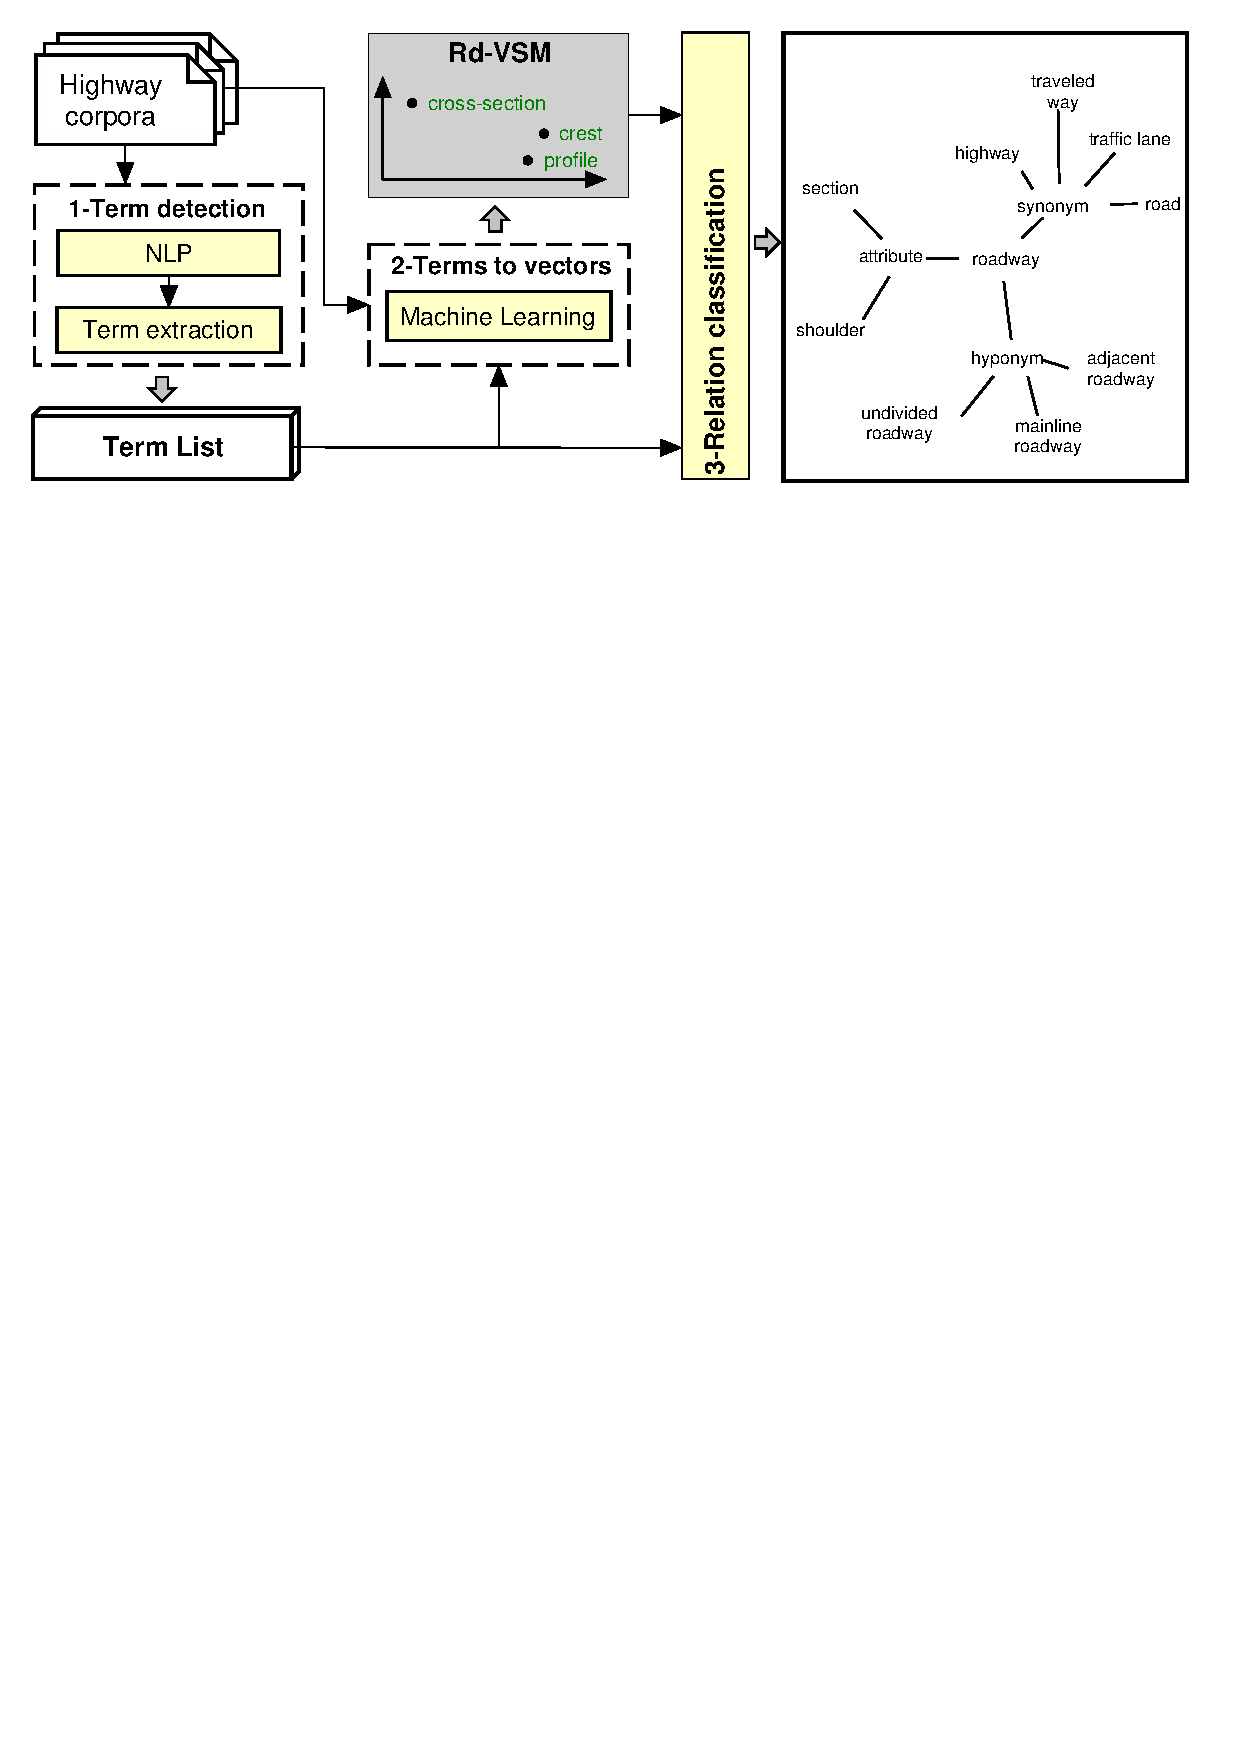
\includegraphics[width=0.95\textwidth]{Figure1_overview_methodology}
	\caption{Overview of the proposed methodology}
	\label{fig:framework}
\end{figure}
%
The goal of this research is to propose an NLP-based methodology that can automate the process of extracting roadway technical terms and their semantic relations from American-English roadway documents. As shown in Figure \ref{fig:framework}, the proposed methodology consists of three major modules that are to: (1) utilize NLP techniques to extract multi-word roadway technical terms from a collected text corpus, (2) train the data obtained form text corpus using the Skip-gram neural network model \cite{mikolov13a} to develop a Roadway Vector Space Model (Rd-VSM) that presents the semantics of roadway terms, and (3) develop an algorithm integrating Rd-VSM and various linguistic patterns to classify relations among technical terms (synonyms, hyponyms and attributes). The below sections discuss these steps in detail.
%
%TODO: The preliminary result is presented by. In this paper, the model is extended with larger training datasets and post-processing to reorganize terms in categories which improves the semantic data searching algorithm.
%
\subsection{Text corpus collection}
%how to collect data, how to clean data to get them ready for training model
%aim text folow remained, flow direction. bottom down, 
%remove heading (chapter, section, subsection), footnote, numerbing, bullets, hyperlink, url, 
In order to develop a domain text corpus for the highway sector, the authors collected a plethora of highway engineering manuals and guidelines from the Federal Department of Transportation (DOT) and from 22 State DOTs. The content of a written guidance document in the engineering field is commonly presented in various formats such as plain text, tables, and equations. Since the structure of words in tables and equations are not yet supported by the state-of-the-art NLP techniques, they were removed from the text corpus. The removal of these features slightly reduces the corpus size, and accordingly affects the training dataset; however, it is necessary since words in tables and equations are not organized in the formal structure of a sentence and therefore the NLP algorithm may extract unreal noun phrases. The final outcome of this phase is a plain text corpus consisting of nearly 16 million words. This dataset is utilized to extract multiple-word technical terms which are then trained and transformed into representation vectors.
%
\subsection{Multi-word terms extraction}
%
\begin{figure}[t]
	\centering
	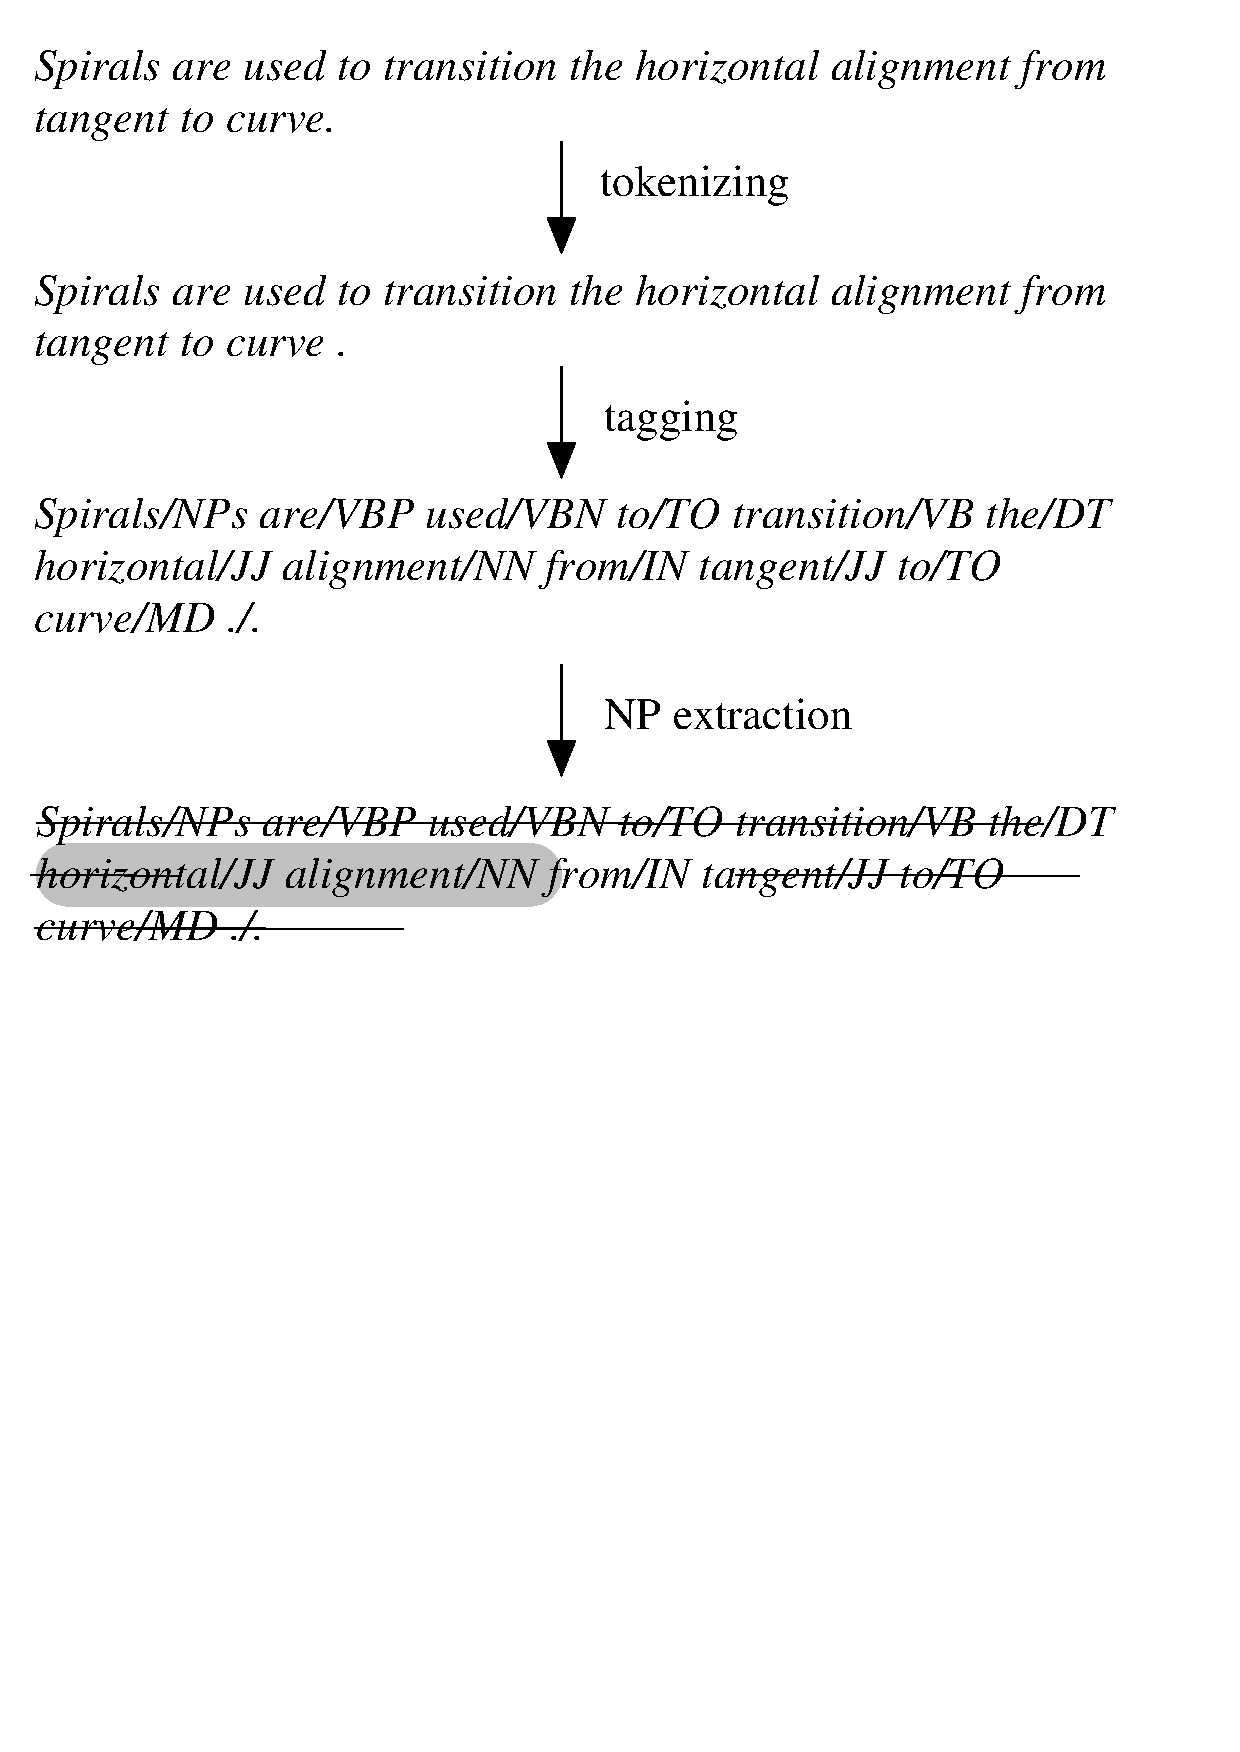
\includegraphics[width=0.45\textwidth]{Figure2_NP_extraction}
	\caption{Linguistic processing procedure to detect NPs}
	\label{fig:np_detect}
\end{figure}
%
Linguists argue that a technical term is either a noun (e.g., road) or a noun phrase (NP) (e.g., right of way) that frequently occurs in domain text documents \cite{justeson95}. The meaning of a multi-word term may not be directly interpreted from the meanings of its constituents; therefore, it must be treated as an individual word.  To ensure that, multi-word terms in the corpus need to be detected and replaced with connected blocks of their members. As mentioned, a multiple-word term must be a noun phrase; thus, noun phrases will be good multi-word term candidates. To detect this type of terms, the corpus is first scanned to search for NPs; and the importance of each of these NPs is then evaluated based on the statistics of occurrence frequencies. The process of extracting multi-word terms is discussed in detail as follows.  %
\subsubsection{Noun phrase extraction}
%
This research implements the Apache OpenNLP package to find sequences of words that match pre-defined noun phrase patterns. Figure \ref{fig:np_detect} illustrates how noun phrases are extracted from the corpus of highway technical documents. This process includes the following steps. %
%
\begin{enumerate} [label=\roman*]
\item Word tokenizing: In this step, the text corpus is broken down into individual units (also called tokens) using OpenNLP Tokenizer.
\item Part of Speed (POS) tagging: The purpose of this step is to determine the Part of Speech (POS) tag (e.g., NN-noun, JJ-adjective, VB-verb, etc.) for each unit of the tokenized corpus obtained from the previous step. A full set of POS tags can be found in the Penn Treebank \cite{marcus93}.
\item Noun phrase detection: Table \ref{table:term_filter} presents the proposed extraction patterns which are modified from the filters suggested by \citeN{justeson95} to extract NPs. The tagged corpus is thoroughly scanned to collect sequences matching those patterns. 
	%
In addition, in order to reduce the discrimination between the syntactic variants of the same term, the collected NPs need to be normalized. The following discuss two types of syntactic variants considered and the proposed normalization methods.
\begin{table} [t]
		\caption{Term candidate filters}
		\label{table:term_filter}
		\centering
		\small
		\renewcommand{\arraystretch}{1.25}
		\begin{tabular}{l l}
			\hline
			\textbf{Pattern} & \textbf{Examples}\\
			\hline
			(Adj|N)*N		& road, roadway shoulder, vertical alignment\\
			(Adj|N)*N Prep (of/in) (Adj|N)*N	&	right of way, type of roadway\\
			%(Adj|N)* 'and/or' (Adj|N)*N & vertical and horizontal alignment\\
			\hline
			\multicolumn{2}{l}{\textit{Note:} |, * respectively denote `and/or', and `zero or more'.  } \\
			\hline
		\end{tabular}
		\normalsize
\end{table}
	%
\begin{itemize}
		\item Type 1 - Plural forms, for example `roadways' and `roadway'. Stemming is a popular process to reduce words to their stems. Despite the fact that, none of the existing algorithms can completely eliminate the errors of over and under stemming, they are good enough to not degrade the overall performance of NLP application \cite{jivani2011stemmer}. This study implements the Pling stemmer \cite{suchanek2006stemmer}, which stems an English noun to its singular form, to normalize plural nouns in the corpus. One advantage of this algorithm is the utilization of both syntactic rules and the vocabulary in a dictionary; hence the miss- or over-stemming errors that take off a true suffix can be reduced. 
		%In order to avoid the effect on other parts such as adjectives (JJ tokens) of a noun phrase, stemming is applied only to the tokens tagged with NNS (plural nouns). 
		%an alternative algorithm is \cite{porter80}, which can allow for automated removal of suffixes. Pling stemmer \cite{suchanek2006stemmer}, 
		%todo: update algorithm so that stemming only occur in the the noun phrase extraction phase, not for the entire corpus.
		\item Type 2 - Preposition noun phrases, for example `type of roadway' and `roadway type'. In order to normalize this type of variant, the form with preposition is converted into the non-preposition form by removing the preposition and reversing the order of the remaining portions. For instance, `type of roadway' will become `roadway type'.
\end{itemize}
\end{enumerate}
%
\par
The first column in Table \ref{table:term_evaluation} represents several examples of the NP bag retrieved from this phase. Since an NP is not certainly a technical term, those that are clearly unlikely to be a term should be excluded from the candidate list. A basic indicator is the occurrence frequency of NPs as a technical term tends to repeatedly occur in domain text documents. To eliminate `bad' candidates, a threshold of frequency can be applied. If users choose a high threshold, rare terms would not be captured. This issue can be addressed when the corpus size is extended. In our experiment, with a frequency threshold of 2, the final list of NPs consists of 112,024 items; and it drops to 8,922 when a threshold of 50 is used. Since this research aims at common technical terms, the authors used a threshold of 50 to remove possibly meaningless term candidates. 
%	
\subsubsection{Multi-word term candidate ranking and selection} 
%
Multi-word term definition varies between authors, and there is a lack of formal and widely accepted rules to define if an NP is a multi-word term \cite{frantzi20}. There are a number of methods proposed for estimating termhood (the degree that a linguistic unit is a domain-technical concept), such as TF-IDF \cite{sparck72,salton88}, C-Value \cite{frantzi20}, Termex  \cite{sclano07}. These methods are based on the occurrence frequencies of NPs in the corpus. Among these methods, Termex outperformed other methods on the Wikipedia corpus, and C-Value was the best on the GENIA medical corpus \cite{zhang08}. This result indicates that the C-value method is more suitable for term extraction from a domain corpus rather than a generic corpus. For this reason, the C-value has been widely used to extract domain terms in the biomedical field, for instance studies performed by \citeN{ananiadou20}, \citeN{lossio13}, and \citeN{nenadic02}. Since the corpus used in this study was mainly collected from technical domain documents, C-value would be the most suitable for the termhood determination task. The C-value measure, as formulated in Equation \ref{eq:cvalue}, suggests that the longer an NP is, the more likely that is a term; and the more frequently it appears in the domain corpus, the more likely it will be a domain term.
	% 
	\begin{equation}
	C-value(a)=
	\begin{cases}
	log_2|a|.f(a), & \text{if a is not nested} \\
	log_2|a|(f(a)-\frac{1}{P(T_a)}\sum_{b\in T_a} f(b)), & \text{otherwise}
	\end{cases}
	\label{eq:cvalue}
	\end{equation}
	%
	Where:
	\begin{description}
		\item[a] is a candidate noun phrase
		\item[|a|] is the length of noun phrase \textit{a}
		\item[f] is the frequency of \textit{a} in the corpus
		\item[Ta] is the set of extracted noun phrases that contain \textit{a}
		\item[P(Ta)] is the size of Ta set.
	\end{description}

%
\par
The term extraction process above results in a dataset containing the detected terms along with their c-value termhood scores. These term candidates are ranked by C-value, and the ones that have negative C-values are discarded.
\par
To automatically remove candidates that are unlikely to be real terms, a threshold C-value can be used. However, doing this may eliminate the real terms that appear in the bottom due to their low frequencies. Manual evaluation of the entire candidate list would avoid the removal of real terms with low C-values. To minimize both laborious work and the number of true terms wrongly discarded, the authors suggest the following method to identify the threshold value. The ranked list of candidates is divided into groups of around 200 items. A graduate student with a civil engineering background was asked to utilize a bottom-up approach to evaluate group by group and stop at which the percentage of actual terms achieved 80 percent. Users can choose a higher percentage limit in cases that the accuracy is critical. This will increase manual evaluation effort. Table \ref{table:term_evaluation} illustrates the evaluation results for several excerpts of the extracted term candidates. The precision values, which represent the percentages of real terms in these groups, are presented in Figure \ref{fig:term_precision}. As shown in the figure, precision values are less than 80 percent for groups with c-values less than 50. This value is set as the threshold for the acceptance of term candidates. The final selected list is comprised of nearly 8,000 multi-word roadway technical terms. 
%To calculate the recall value, expert is required to final all true terms from the corpus \cite{frantzi20}. with the large corpus in this research, it is impossible to do this task. 
%
\begin{table} [t]
	\caption{Excerpts of the extracted candidate terms}
	\label{table:term_evaluation}
	\centering
	\small
	\renewcommand{\arraystretch}{1.25}
	\begin{tabular}{l l l}
		\hline
		\textbf{Term candidate} & \textbf{Termhood} & \textbf{real term?}\\
		\hline
		sight distance		& 9435.314 & yes\\
		design speed & 9052.556 & yes \\
		additional information & 1829.0 & no\\
		typical section & 1801.0  & yes\\
		basis of payment & 1762.478 & no\\
		\hline
	\end{tabular}
	
	\normalsize
\end{table}

\begin{figure}[t]
	\centering
	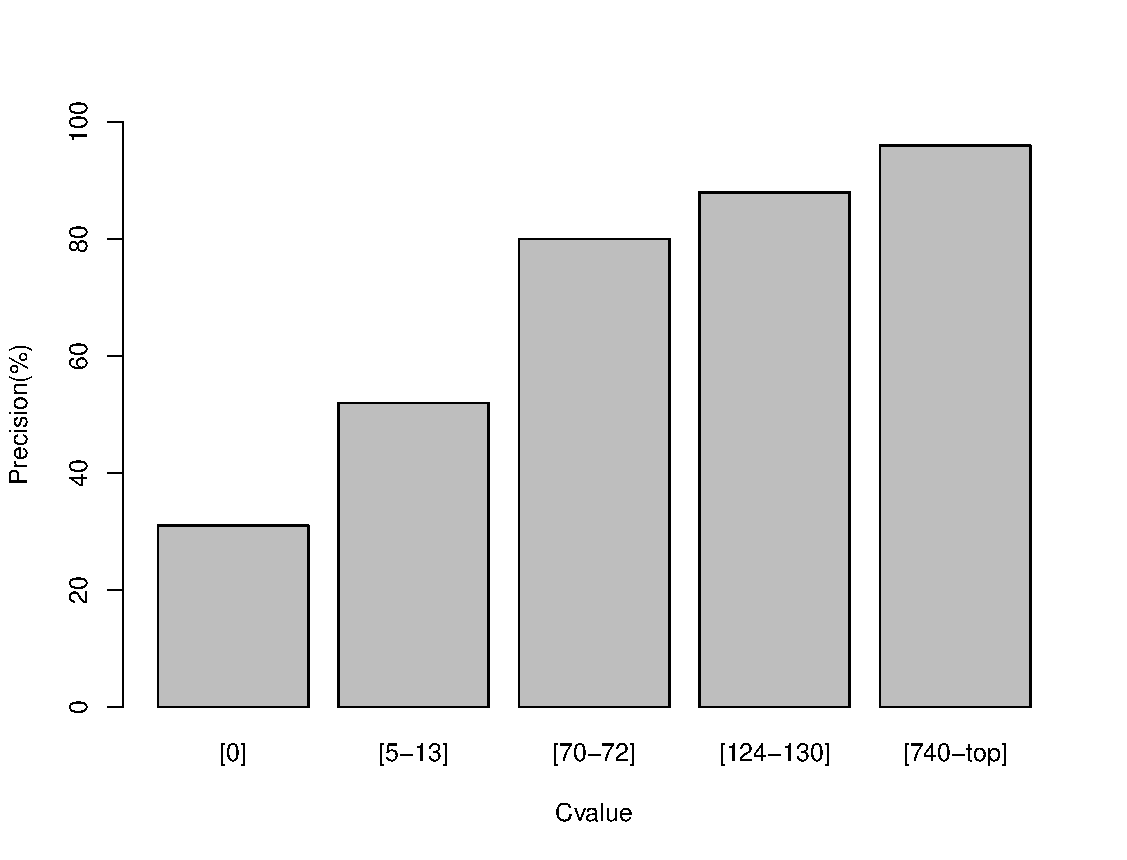
\includegraphics[width=0.5\textwidth]{Figure3_term_precision}
	\caption{Multi-word term extraction evaluation}
	\label{fig:term_precision}
\end{figure}
%
\subsection{Construction of term space model}
%
This step aims at converting the vocabulary in the roadway corpus into a vector space model, namely Rd-VSM. Skip-gram \cite{mikolov13a}, which is an un-supervised machine model, is employed to learn the semantic similarity among words in the text corpus. The Skip-Gram model requires a set of training data in which the input data is a linguistic unit (word or term), and the output data is a set of context words that appear around the target input unit in the corpus. In order to collect this training dataset, the tokenized and stemmed highway corpus is scanned to capture instances of terms and their corresponding context words. Each occurrence of a word will correspondingly generate a data point in the training dataset.
\par
Before collecting the training dataset, an additional step is needed to handle the issue related to multi-word terms. Since document scanning is on a word-by-word basis, the corpus must be adjusted so that multi-word terms can be treated as single words. To fulfill that requirement, the white spaces within a multi-word term are replaced with minus (-) symbols to connect its individual words into a single unit. For instance, `vertical alignment' becomes `vertical-alignment'.
\par
The number of context words to be collected is dependent on the window size that limits how many words to the left and the right of the target word. In the example sentence below, the context of the term `roadway' with the window size of 5 will be the following word set \{bike, lane, width, on, a, width, no, curb, gutter\}. Any context word that is in the stop list (the list that contains frequent words in English such as `a', `an', and `the' that have little meaning) will be neglected from the context set.
%
\begin{center}
	"The minimum [bike lane width on a \underline{roadway} with no curb and gutter] is 4 feet ."
\end{center}

%skip-gram model
%how to modify the method of selecting conext words
%java program
%
\begin{figure}[t]
	\centering
	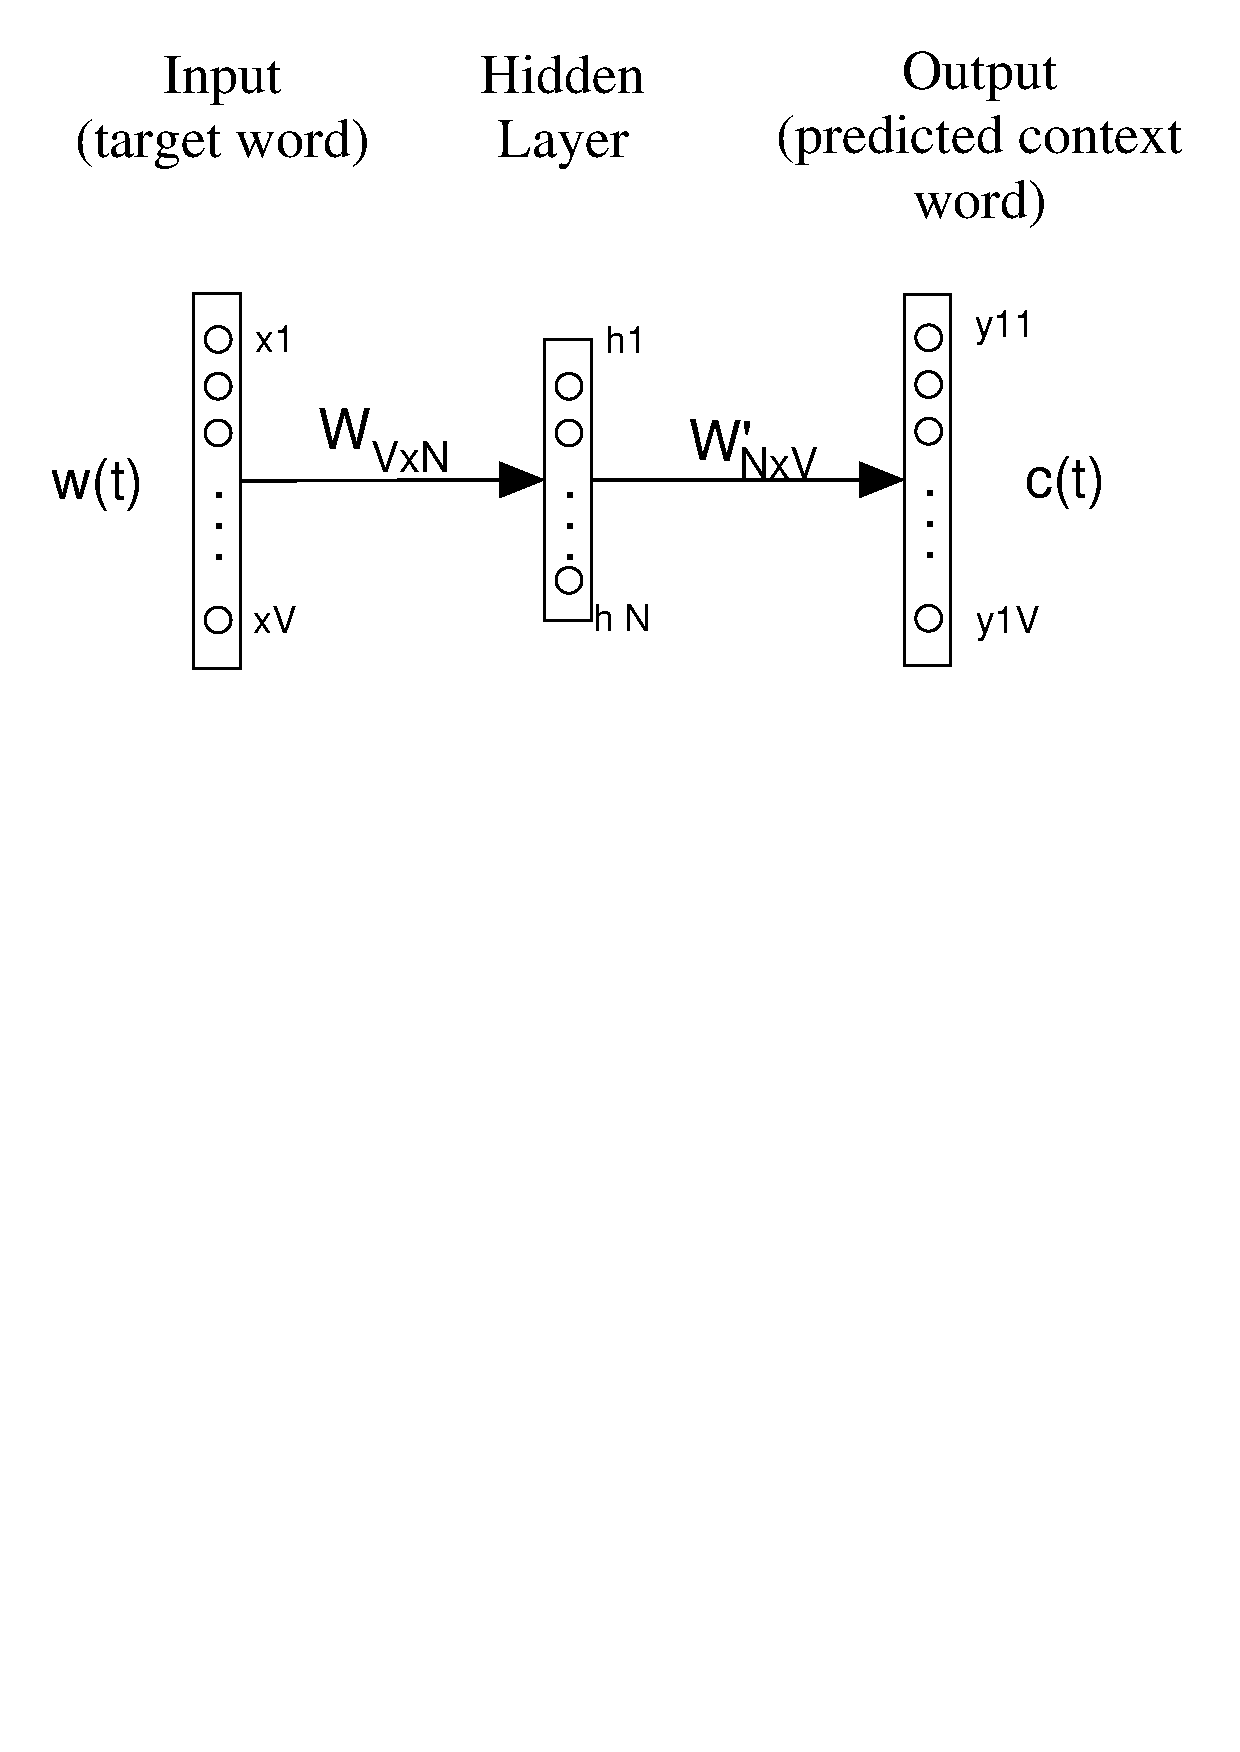
\includegraphics[width=0.45\textwidth]{Figure4_skip-gram-model}
	\caption{Skip-gram model}
	\label{fig:skip-gram}
\end{figure}
%
The semantic similarity is trained using the Word2Vec module in the Apache Spark MLlib package \cite{apache16}, an emerging open-source engine, which is based on the Skip-gram neural network model \cite{mikolov13a}. Figure \ref{fig:skip-gram} illustrates the learning network when the context set includes only one word, where \textit{V} and \textit{N} respectively denote the corpus vocabulary and hidden layer size. In this model, a word in the corpus vocabulary is encoded as a `one-hot' vector which is a vector in which only one element at the index of the word in the vocabulary is set one, and all other items are zero. For example, the one-hot vector of $k^{th}$ word in the vocabulary with the size of V will be $\{x_1=0, x_2=0, ..., x_k=1,...x_V=0\}$. The outcome of this machine learning process is a set of word representation vectors in an N-dimension coordinate system. The similarity among these vectors represents the similarity in context between the corresponding words. The bullets below explain how the predicted context vector of $k^{th}$ word is computed using the parameter matrices resulted from the learning process. As we can see, the similarity between two predicted context vectors depends only on the similarity between their corresponding input representation vectors; thus, these vectors are used to represent the semantics of  words. 
%
\begin{itemize}
	\item $k^{th}$ word: $[x_k]_{1.V} = [x_1=0, x_2=0,...,x_k=1,..., x_V=0]$ which is an one-hot vector.
	\item Hidden vector: $[h]_{1.N} = [x_k]_{1.V}.W_{V.N} = [w_{k1},w_{k2},..., w_{kN}]= v_{wk}$ which is equivalent to the $k^{th}$ row of the W matrix since the input vector is a `one-hot' vector. The $v_{wk}$ vector is called the input \textit{representation vector} of the $k^{th}$ word.
	\item Predicted context vector: $[y_k]_{1.V} = v_{wk}.W'_{N.V}$. 
\end{itemize}
%
\par
The learning model includes three major parameters that are \textit{frequency threshold}, \textit{hidden layer size} and \textit{window size} (see Table \ref{table:nn-parameters}). To eliminate those data points with low frequencies of occurrence that are unlikely to be technical terms, Word2Vsec allows for the use of \textit{frequency threshold}. Any word with the rate lower than the limit will be ignored. \citeN{rehurek14} suggests a range of (0-100) depending on the data set size. Setting this parameter high will enhance the accuracy, but many true technical terms would be out of vocabulary. A preliminary study based on the preliminary corpus with only several millions of words shows that with the frequency of 20, there are very few non-technical terms involved in the training dataset. Hence, with the larger dataset to be collected, this parameter can be higher and up to around 50. The second important parameter is \textit{layer size} which determines the number of nodes in the hidden layer. This parameter highly affects the training accuracy and processing time. A larger layer size is better in terms of accuracy, but this will be paid off by the running time. A reasonable figuration for this parameter is from tens to hundreds \cite{rehurek14}. The final major parameter, \textit{context window size}, decides how many context words to be considered. Google recommends a size of 10 for the Skip-gram model \cite{google2016}. These parameters are subject to be changed so that the best model can be achieved. The effects of these parameters on the model performance are discussed in Section \ref{sec:eval_RoadLex}.
%
\begin{table} [t]
	\caption{Skip-gram model parameters}
	\label{table:nn-parameters}
	\centering
	\small
	\renewcommand{\arraystretch}{1.25}
	\begin{tabular}{l l}
		\hline
		\textbf{Parameter} & \textbf{Value}\\
		\hline
		Frequency threshold & 50-100\\
		Hidden layer size		&	100-500\\
		Context window size	&	5,10,15\\
		\hline
	\end{tabular}
	\normalsize
\end{table}
%
\par
Figure \ref{fig:hvsm} presents the Rd-VSM vector space model derived from the training process when the parameters, \textit{frequency threshold}, \textit{hidden layer size} and \textit{window size} are set 50, 300 and 10 respectively. In this model, each word in the highway corpus is represented as a vector in a high dimensional space. Since the representation vectors are in a multi-dimensional space; to present the space in 2D graph, PCA (Principle Component Analysis) is used to reduce the dimension size to two.
\par
The similarity between terms in the Rd-VSM model can be measured by the angle between two word representation vectors (Equation \ref{equ:cosin_sim}) or the distance between two word points (Equation \ref{equ:dis_sim}). Figure 5 illustrates the clustering of terms by their distances. In this figure, an \textit{inlet} can be inferred to be more similar to an \textit{outlet} (blue) than a \textit{sidewalk} (green). Using this technique, the most similar terms for a given term can be obtained. Table \ref{table:nearest_example} shows a partial ranked list of the nearest terms of `roadway' in order of similarity score.
%
\begin{figure}[t]
	\centering
	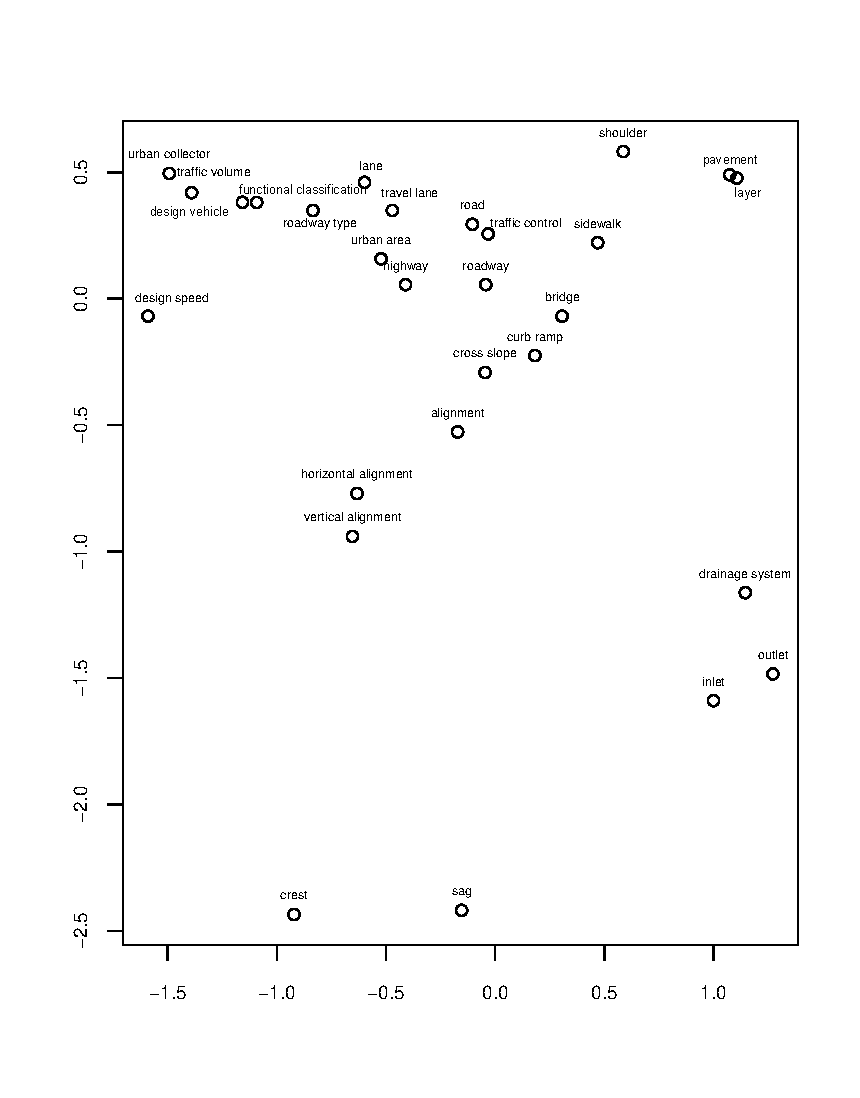
\includegraphics[width=0.95\textwidth]{Figure5_hvsm_space}
	\caption{Highway term space model (Rd-VSM)}
	\label{fig:hvsm}
\end{figure}
%
\begin{equation}
\label{equ:cosin_sim}
cosine\_similarity = \frac{A \cdot B}{||A|| \cdot ||B||}
\end{equation}
%
\begin{equation}
\label{equ:dis_sim}
dis\_similarity =\sqrt{(xA_1-xB_1)^2+(xA_2-xB_2)^2+...+(xA_n-xB_n)^2}
\end{equation}

Where: n is the hidden layer size.
%
\begin{table} [t]
	\caption{Examples of top nearest words}
	\label{table:nearest_example}
	\centering
	\small
	\renewcommand{\arraystretch}{1.25}
	\begin{tabular}{l l l  l}
		\hline
		\textbf{Term} & \textbf{Nearests} & \textbf{Cosine} &\textbf{Rank}\\
		\hline
		roadway			& highway & 0.588 & 1\\
		& traveled-way & 0.583 & 2\\
		& roadway-section & 0.577 & 3\\
		& road & 0.533 & 4\\
		& traffic-lane & 0.524 &5\\
		& separating & 0.522 &6\\
		& adjacent-roadway & 0.519 & 7\\
		& travel-way & 0.517 & 8\\
		& entire-roadway & 0.513 & 9\\
		& ...&...& ...\\
		& roadway-shoulder & 0.505 & 12\\
		& roadway-cross-section & 0.491 & 18\\
		& undivided & 0.452 & 37\\
		& mainline-roadway & 0.450 & 42\\
		\hline
	\end{tabular}
	\normalsize
\end{table}

\subsection{Semantic relation classification}
The purpose of this module is to design an algorithm for automated classification of the semantic relations among the roadway technical terms. This study considers three core relation types of a semantic resource that are: synonym (meaning equivalence), hypernym-hyponym (also known as IS-A or parent-child relation), attribute (concept property) \cite{jiang1997semantic,lee13}. The following are the fundamental ideas behind the designed algorithm. Two terms that relate to each other through these semantic relations would have a high similarity score. Therefore, the top nearest terms resulted from Rd-VSM would be a great starting point for detecting relations between technical terms. For example, in the list of the nearest terms of `roadway' (see Table \ref{table:nearest_example}), true synonyms are `highway' (rank 1), `traveled-way' (2) and `road' (4); attributes include `roadway-section' (3), `roadway-shoulder' (12); and `adjacent-roadway' (7) and `undivided' (37) are hyponyms which show different types of roadway.
\par
Algorithm \ref{alg:term_class} shows the designed pseudo code for classifying the nearest terms of a given target term. The algorithm utilizes linguistic rules and clustering analysis to organize the nearest list into the following three groups: (1) attribute, (2) hyponym, and (3) synonym. The algorithm first detects terms belonging to the first two categories using linguistic patterns, and employs cluster analysis for the last group.
%
\subsubsection{Attributes and hyponyms}
The filter rules to detect these relations are presented in Table \ref{table:attribute_pattern}. For a multi-word term matching pattern 1, we can infer that \textit{Noun1} is an attribute of concept \textit{Noun2}; and \textit{Noun2} is an attribute of \textit{Noun1} in the pattern 2. Pattern 3 is for detecting hyponyms where the matched NP is a hyponym of its \textit{Noun2} component.  
  %
\subsubsection{Synonyms}
After the words in the first two categorized are classified, the remained nearest words will fall into the third group. However, some of them may have far or even no relation with the target word. In order to address this issue, this framework employs the K-mean clustering algorithm \cite{macqueen67} to split the remained list into multiple layers based on the similarity score. The terms in the last layers are unlikely to be a synonym; and thus, are removed from the classified list. Only the terms in the top cluster are kept and categorized as synonyms. 
\par
By the end of the synonym recognition phase, the algorithm will generate a list of classified nearest terms. Table \ref{table:term_clustering} shows one example of the output generated by the algorithm. 
%In contrast, since synonym recognition is well known as the process of evaluating the sharing of common attributes, hypernyms, and hyponyms, this process will rely on the results from the detection of other relations. This task will first detect the following relations (hypernyms, hyponyms and attributes) and then use them as features to find synonyms.
%
\begin{algorithm}[h]
	
	\caption{Semantic relation classification algorithm}\label{alg:term_class}
	\begin{algorithmic}[1]
		\State \textbf{Inputs}: term \textit{t}, list of nearest terms \textit{N}, full list of terms \textit{F}
		\State \textbf{Output:}: Classified list of terms \textit{C}
		\Procedure{Term classification procedure}{}
		%\State $\textit{n} \gets \text{size of }\textit{W}$
		%\State $\textit{m} \gets \text{size of }\textit{T}$
		\State $\textit{Att} \gets \text{list of attributes}$
		\State $\textit{Hyp} \gets \text{list of hyponyms}$
		\State $\textit{Syn} \gets \text{list of synonyms}$
		\State $\textit{w} \gets \textit{null}$
		\ForAll {$n \in N$}
		\If {$n$ contains \textit{t}}
		\State $w \gets n$
		
		\Else
		\ForAll {$f \in F$}
		\If {$f$ contains both $n$ and \textit{t}}
		\State $w \gets f$	
		\State Break for
		
		\EndIf
		\EndFor
		\EndIf
		
		\If {$w$ matches \textit{Attribute pattern}}
		\State add $w$ to \textit{Att}
		\ElsIf {$w$ matches \textit{Hyponym pattern}}
		\State add $w$ to \textit{Hyp}
		\Else
		\State add $w$ to \textit{Syn}
		\EndIf
		\EndFor
		\State Cluster \textit{Syn} and discard low relevant terms
		
		\EndProcedure
	\end{algorithmic}
\end{algorithm}
%
%\subsection{Attribute and hyponym patterns}
%
\begin{table} [t]
	\caption{Patterns to extract attributes and hyponyms}
	\label{table:attribute_pattern}
	\centering
	\small
	\renewcommand{\arraystretch}{1.25}
	\begin{tabular}{l l l}
		\hline
		\textbf{Relation} & \textbf{Pattern} & \textbf{Example}\\
		\hline
		Attribute &	Noun1 of Noun2 & the width of the road\\
		& Noun1 Noun2	&	road width, project cost\\
		Hypernym-hyponym & Noun1 Noun2 & vertical alignment isA alignment\\
		\hline
	\end{tabular}
	\normalsize
\end{table}
%
%After the candidate list is refined, the frequency of occurrence for each candidate will then be used to compute the degree that term 'a' is an attribute of concept 'c'. If 'a' is a typical attribute of 'c', it should frequently occur in the corpus. Each concept 'c' will correspondingly have a list of attribute candidates (called list A) and their frequency of occurrences. The likelihood that 'a' is an attribute of concept 'c' is estimated using the normalized probability formula (see Equation \ref{eq:attribute}). The attribute candidates for each concept will be ranked by the likelihood measure and the top list over a threshold value will be accepted as typical attributes. 
%\begin{equation}
%P(a|c)=\frac{n(c,a)}{\sum_{a* \in A} n(c,a)}
%\label{eq:attribute}
%\end{equation}
%\subsection{Synonym/sibling and functional relation recognition}

%
\begin{table} [t]
	\caption{An example in RoadLex}
	\label{table:term_clustering}
	\centering
	\small
	\renewcommand{\arraystretch}{1.25}
	\begin{tabular}{l l l l l}
		\hline
		\textbf{Term}	&\textbf{Relation Group}	& \textbf{Nearests} & \textbf{Cosine} & \textbf{Rank}\\
		roadway			&Synonym					& highway & 0.588 & 1\\
		&							& traveled-way & 0.583 & 2\\
		&							& road & 0.533 & 4\\						
		&							& traffic-lane & 0.524 &5\\ 						
		&							& travel-way & 0.517 & 8\\  \cmidrule{2-5}
		&Attribute					& separating & 0.522 &6\\
		&							& roadway-section & 0.577 & 3\\						
		&							& roadway-shoulder & 0.505 & 12\\
		&							& roadway-cross-section & 0.491 & 18\\\cmidrule{2-5}						
		&Hyponym					& adjacent-roadway & 0.519 & 7\\
		&							& entire-roadway & 0.513 & 9\\
		&							& undivided & 0.452 & 37\\
		&							& mainline-roadway & 0.450 & 42\\
		\hline
	\end{tabular}
	\normalsize
\end{table}


\section{Performance evaluation} \label{sec:eval_RoadLex}
%evaluation method
This section presents a performance evaluation of the proposed system on the ability to identify synonyms. In this experiment, a gold standard is used. The gold standard consists of 70 sets of synonyms (both single and multi-word terms) which were examined and extracted from a Wikipedia transportation glossary \cite{wikipedia16}. The developed algorithm was employed to find the synonym for a given input term. The automatically identified synonym is the nearest word in the synonym lexical group. The evaluation outcome returns ``true'' if the automatically identified synonym belongs to the actual synonym set of the tested term in the golden standard, or ``false'' if it does not. The answer will be ``N/A'' if the target term is out of the model vocabulary. The performance was evaluated using the following three measures including precision, recall, and f-measure. Precision refers the accuracy in the conclusions made by the system, and recall reflects the coverage of domain terms of the system. The F score, which is a combined measure of precision and recall, presents the overall performance of a system. 
%
\begin{align} 
&Precision = \frac{\text{number of correctly detected synonyms}}{\text{total detected synonyms}}  \\
&Recall = \frac{\text{number of correctly detected synonyms}}{\text{total tested terms}}  \\ 
&F-measure = \frac{2.Precision.Recall}{Precision+Recall}
\end{align}
%results
\begin{table} [b] 
	\caption{Performance of the synonym matching task with various training settings}
	\label{table:eval_syn_par_effect}
	\centering
	\small
	\renewcommand{\arraystretch}{1.25}
	\begin{tabular}{l l l l l }
		\hline
		\hline
		\textbf{Parameter changed} & \textbf{Model} & \textbf{Precision (\%)}  & \textbf{Recall(\%)} & \textbf{F (\%)}\\
		\hline
		Baseline	&	50-100-5	&79		&53		&63\\
		\hline
		\textbf{Window size}	&\textbf{50-100-\underline{10}}	&\textbf{81}		&\textbf{54}		&\textbf{65}\\
		&50-100-\underline{15}	&81		&54		&65\\
		\hline		
		Frequency threshold	&\underline{75}-100-5	&74		&50		&60\\
		&\underline{100}-100-5	&77		&51		&62\\
		\hline
		Hidden layer size	&50-\underline{200}-5	&79		&53		&63\\
		\hline
		\hline
	\end{tabular}
	\normalsize
\end{table}
%
%synonym matching peformance result
Table \ref{table:eval_syn_par_effect} shows the performance with various training model settings. The parameters of the baseline model are 50, 100 and 5 respectively for frequency threshold, hidden layer and window size. The authors changed the configuration of these parameters one by one to evaluate their effects to the model performance. While changing a certain parameter, other parameters are kept unchanged compared to their values in the base model. As presented in the table, the model performance is not significantly sensitive to the changes of training parameters. The increase of window size to 10 or 15 resulted in the best model which has a precision of 81\% and an F-measure of 65\%. The changes of other parameters did not improve the performance. Especially, the increase of frequency threshold value has negative impact. This result confirms the reasonable selection of the frequency threshold to eliminate unlikely term candidates in the NP extraction phase.
%compared to the previous publication by the authors, this algorithm has been improved with significantly higher accuracy. the post-processing is one reason for the out-performance of the proposed method.  
%
%result
\begin{table} [b] 
	\caption{Comparison of synonym matching performance between WordNet and RoadLex}
	\label{table:eval_syn_vs_Wordnet}
	\centering
	\small
	\renewcommand{\arraystretch}{1.25}
	\begin{tabular}{l l l l }
		\hline
		\hline
		\textbf{Lexicon} & \textbf{Precision (\%)}  & \textbf{Recall(\%)} & \textbf{F (\%)}\\
		\hline
		Wordnet	&76 	&40 	&52\\	
		\textbf{Proposed system} &\textbf{81}	&\textbf{54}		&\textbf{65}\\	
		\hline
		\hline
	\end{tabular}
	\normalsize
\end{table}
\par
The proposed model was also compared with the generic WordNet database. Table \ref{table:eval_syn_vs_Wordnet} presents the comparison of performance between the proposed framework (with the 50-100-10 setting) and WordNet. As shown, the present system outperforms WordNet in all measures, and the combined F-measure is significantly improved (65\% compared to 52\%). The biggest contribution to the improvement of the overall F-measure is the recall value which represents a better coverage of roadway vocabulary. 
%attribute  hyponyms and attributes. finding performance
%for attribute and hyponym only precision is determined. to determine the recall require of all possible true attributes for a concept which is challenging and unrealistic task, this research evaluate the accuracy of the extracted attributes. this largely depend on the size and the variety of discipiline covered in the corpus. select of one in each set of synonyms in the gold standard and  humam evaluate attribute and non-attribute. the performance in measure using Equation which represent the percentage of correctly extracted attribute/hyponym. 

%
\section{Discussions} \label{sec:dis}
%contribution of the research
This paper proposes an NLP based methodology to assist professionals in extracting roadway terms and their semantic relations from text documents. A key contribution to the body of knowledge is the novel framework with a new algorithm that allows for automated detection of technical terms and their relations without reliance on existing hand-coded dictionaries as used by previous researchers such as \citeN{zhang16}. The present framework is not to completely eliminate the human interfere, but is expected to become an enabling tool that can help researchers in the domain quickly develop supporting ontologies and other forms of semantic resources for their specific use cases. With respects to the facilitation of semantic interoperability for the infrastructure sector, the implications of this study would accelerate the process of removing the current bottleneck in extensive machine readable dictionaries which are required for an unambiguous data sharing, integration or exchange. 
%potential application
%todo: refer two research related to NLP in which the first step is to develop lexicon, or other semantic similarity algorithm.
\par
The semantic similarity model and the relation classification algorithm developed in this study are expected to become fundamental resources for a variety of NLP related studies in the highway domain. NLP based platforms can utilize these resources for term sense analysis which is crucial for text mining to extract meaningful information from text documents, information retrieval, or natural language based human-machine interaction. Some specific examples of these potential applications are as follows. Information retrieval systems can use the semantic relations provided by the algorithm to classify project documents by relevant topics by analyzing the relatedness between the index keywords in those documents. In addition, questionnaire designers can utilize the system to search for synonyms so that appropriate terms can be selected for specific groups of potential respondents who might be from multiple disciplines or regions. Another application is that the query systems for extracting data from 3D engineered models would be able to find alternative ways to query data when users' keywords do not match any entity in the database. Since users have different ways and keywords to query data, the ability to recognize synonyms and related concepts of a query system would provide flexibility to the end user. Also, the synonym detection function would enable the matching data items such as (e.g., cost, productivity, etc.) when integrating data from distinct departments or states to develop a national database. This study is also expected to fundamentally transform the way human interacts with a machine as technical terms which are a basic unit of human language can be precisely understood by computer systems. Instead of using computer languages, the end user can use natural language to communicate with computer systems.
%add discussions
%In order to enable computer to understand human language, a machine-readable dictionary which defines meanings of relevant vocabulary is required. therefore, the developed lexicon can be used by NLP applications for the domain of infrastructure. 
\par
%
%limitation and potential direction for improvement
The current study has a number of limitations. First, the highway corpus is still relatively small with only 16 million words, compared to the corpus sizes in other domains with billions of words. Since the recall value largely depends on the corpus size, the expansion of the highway corpus size by adding more documents from other state agencies and disciplines (e.g., survey, construction, operation and maintenance) would enable more technical terms to be covered in the vector space model; and consequently, the recall would be improved. Secondly, the number of semantic relation categories is limited to only three types of relations that are attributes, hyponyms and synonyms. There are other important semantic relations that are not considered such as hypernyms, siblings, functional associations, etc. Including these relations would enhance the precision value when incorrect answers such as saying a functionally associated term is a synonym can be reduced. Third, this study only targets at the synonymy issue, the issue of polysemy is not yet addressed. Further research is needed to detect different senses of a roadway term. One potential solution is to apply cluster analysis on the instances of context to determine the possibility that a term would have multiple meanings. %
%add limitation
%todo: discussion on what is a good precision and f-measure 
\section{Conclusions} \label{sec:conclns3} 
Data manipulation from multiple sources is a challenging task in highway asset management due to the inconsistency of data format and terminology. The contribution of this study is an NLP-based approach to automated classification of semantic relations among roadway technical terms based on their word occurrences in the domain text documents. This research employs advanced NLP techniques to extract technical terms from a highway text corpus which is composed of 16 million words built on a collection of design manuals from 22 State DOTs across the U.S. Machine learning is used to train the semantic similarity between technical terms. An algorithm is designed to classify the nearest terms resulted from the semantic similarity model into distinct groups according to their lexical relationships. 
\par
The developed system has been evaluated by comparing the results obtained from the computational model and a man-crafted gold standard. The result shows an accuracy of over 80 percent. The best model is associated with the training parameters of 50, 100 and 10 respectively for frequency threshold, hidden layer size, and window size. Although a significant improvement is shown in comparison with an existing thesaurus database, the overall performance is not relatively high. This might be due to the size of the training data. Future research will be conducted to expand the highway corpus to further disciplines such as asset management, and transportation operation. 
\par
The proposed methodology for detecting semantic relations, with the enhanced automation and scalability level, is expected to significantly reduce human efforts in developing a semantic resource for a specific use case within the highway domain and become an enabler for semantic interoperability in this domain. The research also opens a new gate for computational tools regarding natural language processing in the highway sector. The developed system would enable computer systems to understand terms and consequently transform the way human interacts with a computer by allowing users to use natural language.

\bibliography{mybib}
%
%
\listoffigures

\end{document}

